\documentclass[12pt]{article}
\usepackage[margin=1in]{geometry}
\usepackage{graphicx}
\usepackage{setspace}
\usepackage{url}

\title{Tecellate: A Distributed Environment for AI Simulations}
\author{
        Steve Johnson (srj15@case.edu)\\
        Case Western Reserve University\\
}
\date{\today}

\begin{document}
\doublespacing
\maketitle

% \begin{multicols}{2}

\section{Introduction}

In recent years, the fields of artificial intelligence and robotics have produced independent robots capable of cooperative behavior, for example the CoDA project\cite{CoDA}. However, there is no general and accessible platform upon which to test the AI required for cooperative behavior. The Tecellate project helps to solve this problem in a small way by providing a distributed grid-based world inhabited by agents with the ability to move, communicate, and be destroyed.

\section{Simulation Rules}
\label{rules}

The simulation is turn-based and runs over a fixed number of turns. At the beginning of each turn, agents receive information about the terrain and other nearby agents. In response, agents can either attempt to move or remain still, as well as simultaneously broadcast a message. When all agents have decided on an action for a turn, the actions are executed and a new turn begins.

\subsection{World and Movement}

The simulation world consists of a $w$x$h$ grid of signed integers. If the number is non-negative, it is the terrain height. Otherwise, the cell is impassable. An agent can move at most one cell up, down, left, or right per turn. The move action takes one extra turn for every absolute height unit difference above 1.

If more than one agent attempt to move into the same cell, they are destroyed.

\subsection{Messages}

An agent may broadcast a message of 1024 bytes or less every turn regardless of any other action it takes. The broadcast system is a simplification of radio communication: nearby agents within a maximum radius will receive the message. Other agents will not hear it.

\subsection{Perception}

Agents are informed of their global position in the world. They are also informed of the position of any agents within a maximum number of cells.

\subsection{Food}

Agents must search the grid to find food. If their coordinator calculates that their food counter is below zero, they disappear from the grid. This rule would give agent programmers incentives to introduce distributed communication networks to inform faraway agents of abundant new food sources.

\section{Usefulness of the Simulation}

The simulation provides a close enough approximation of the real world to allow testing of high-level coordination algorithms to be tested using a very simple API.

The rules for movement (1 delayed turn per cell height difference) and perception provide an opportunity to experiment with pathfinding algorithms in an environment where little information outside a limited area is available, similar to the conditions of the DARPA autonomous vehicle events.

The rules for communication force agents to communicate with distant agents by passing messages through nearby agents, creating ad-hoc wireless networks.


\section{Distributing Work}

Simulating thousands of agents and millions of grid cells simultaneously at a reasonable speed will require multiple machines. One server, the \emph{game coordinator}, will be responsible for starting the game and reporting the rules. The other $n_ac$ servers will be \emph{agent coordinators}, responsible for delivering messages, taking and executing agent orders, and reporting success or failure.

Agents interact in two primary ways: messages and movement conflict/support. Both are only effective within a certain proximity. These properties suggest that agents should be assigned to coordinators based on proximity. There are multiple ways to perform this assignment. This paper will consider three strategies: static assignment, fixed region distribution, and dynamic grid distribution.

\subsection{Static Assignment}

The simplest way to assign agents to coordinators is to assign $\frac{n_agents}{n_ac}$ agents to each agent coordinator at random or based on some positioning heuristic. No agents will ever change their coordinator, but there may be significant overhead from close agents on different coordinators attempting to move and communicate. Also, each agent coordinator will have to be in constant communication with all other coordinators because it cannot know which other coordinators contain agents close to its own.

\subsection{Fixed Region Distribution}

One way to alleviate the communication problem is to assign each agent coordinator a fixed portion of the grid to be responsible for. There will never be a recalculation of bounds and each coordinator has a constant set of neighbor coordinators to communicate with. Each turn, adjacent coordinators will exchange messages, and order confirmations for agents near their shared border, and full agent information transfers for agents moving from one coordinator's region to a neighbor's region.

This strategy requires the least communication between agent coordinators when agents move relatively little, but requires much communication when many agents are near region borders or move between borders often. It also introduces inefficiency in work distribution when disproportionate numbers of agents are gathered in small regions.

\subsection{Dynamic Grid Distribution}

Like fixed region distribution, dynamic grid distribution assigns each agent coordinator a region of the grid to be responsible for. However, the regions themselves are arranged in a meta-grid. This grid arragenement allows rows and columns to be resized while the simulation is running, partially alleviating the work distribution problem.

\subsection{Strategy for First Version}

The initial implementation of Tecellate will use static assignment to test communication protocols and basic mechanics. Then a fixed region distribution over a meta-grid will be introduced. If there is time, dynamic grid distribution will be implemented.

\section{Protocols}

\subsection{Master}

The master process is responsible for connecting to the coordinators, sending them configurations, and waiting for their final responses. Since it needs to complete only a linear sequence of steps, it runs in a single thread.

The master process begins by reading a configuration file with a list of IP addresses and ports at which coordinators can be reached. It also reads data about the world size, terrain, and the locations of agents. It then decides which agents will be managed by which coordinators and which coordinators will be \emph{neighbors}, i.e. which coordinators will maintain connections to each other.

It opens a TCP connection with each coordinator and sends the configuration information, then waits for confirmations from all coordinators that the information was received (\texttt{CONFIG\_CONFIRM}). It then waits for a second confirmation that all agents were launched successfully (\texttt{READY}) and the simulation can begin.

\begin{figure*}
    \begin{center}
        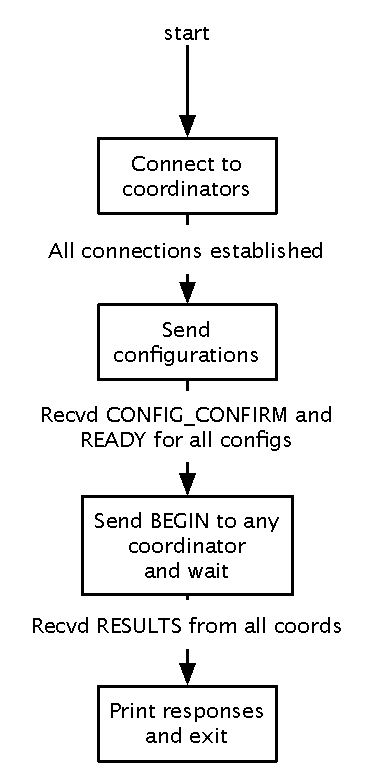
\includegraphics[scale=0.5]{figures/state_master.pdf}
    \end{center}
    \caption{State transition diagram for the master process.}
    \label{master}
\end{figure*}

To start the simulation, the master process sends \texttt{BEGIN} to any coordinator. It then waits for all coordinators to report back to it with information about the end of the simulation (RESULTS). Finally, it prints all relevant results.

A state transition diagram of this process is shown in figure \ref{master}.

\subsection{Coordinator}

The coordinator is the most complex part of the system. At any given time, as many as four threads may be running simultaneously. The full state transition diagram is shown in figure \ref{coord}.

At the high level, the coordinator connects to neighbors and agents, serves requests for information about the state of its agents in the last turn, and processes its own agents by requesting information from its neighbors and from its agents.

\subsubsection{The main thread}

The main thread handles the lifecycle of the coordinator and those of its connections. It begins by listening for a TCP connection from the master process. Once connected, it reads its configuration, which contains IP addresses/ports at which its neighbors are listening for it, which agents it should launch, and where to place them. It sends \texttt{CONFIG\_CONFIRM} back to the master process.

Coordinators are connected to each neighbor by two TCP connections. The coordinator listens on one of these for requests for information from the neighbor. It uses the other to request information of the neighbor. These connections are established using information sent from the master process.

Coordinators are connected to actors by a single TCP connection. To begin the agent communication process, the coordinator launches the agent process and repeatedly tries to open a socket to it until it responds.

The connections to the neighbors and agents are all established at once, asynchronously. When all connections are established, the coordinator sends READY to the master process and launches the \texttt{listenMaster} and \texttt{listenPeers} threads.

It waits for two locks, \texttt{TCOMPLETE1} and \texttt{TCOMPLETE2}, to be released. After these locks are released, the coordinator sends information about the final state of its agents back to the master process and exits, sending exit messages to the agents as well.

\begin{figure*}
    \begin{center}
        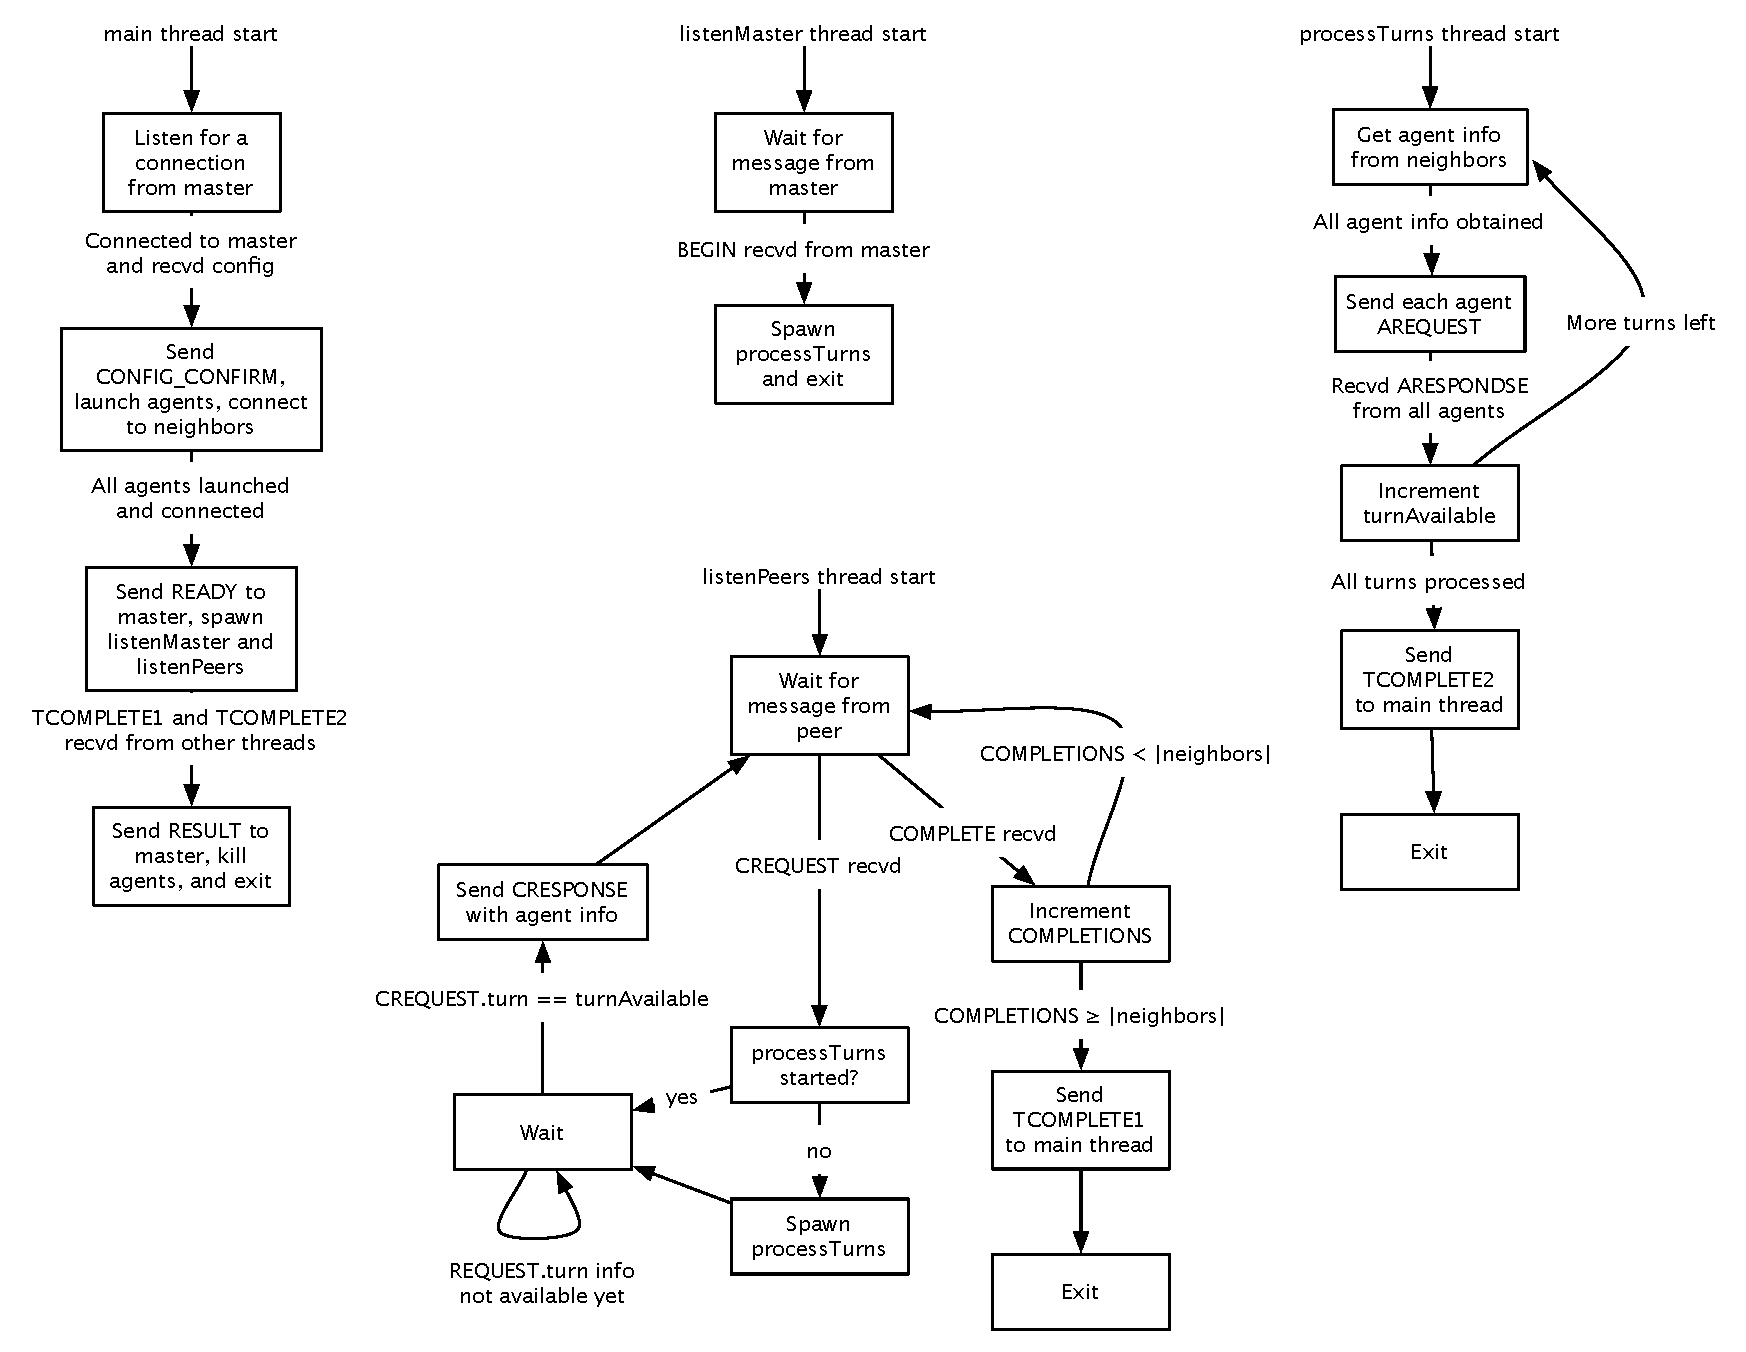
\includegraphics[scale=0.5]{figures/state_coord.pdf}
    \end{center}
    \caption{State transition diagram for the coordinator processes.}
    \label{coord}
\end{figure*}

\subsubsection{The listenMaster thread}

The master process begins the simulation by sending \texttt{BEGIN} to any coordinator. This message is received by the \texttt{listenMaster} thread, whose only job is to spawn the \texttt{processNodes} thread and exit.

\subsubsection{The listenPeers thread}




\section{Future Work}

The most pressing implementation issue is the lack of choice of coordinator assignment strategy. The current version of the system assigns agents to coordinators statically.

To make dynamic reassignment possible, a protocol to transfer ownership of an agent must be designed. The agent must be serialized and shut down, its serialized form must be sent from one coordinator to another, and the new coordinator must start a new process for it.

More work should also go into designing and implementing more predictable failure behavior.

\section{Other Possible Simulation Rules}

The rules outlined in Section \ref{rules} describe a minimal environment to test the utility and efficiency of Tecellate. The rules outlined in this section may add more interesting mechanics to the simulation.

\subsection{Factions}

Agents are not currently identified with a faction and act essentially as free agents. Under faction rules, they would be divided into teams in a competition for survival.

\subsection{More Sophisticated Movement/Death Rules}

In the current version of Tecellate, two agents that move into the same cell are killed. This is a very simplistic rule, and could be replaced with a system of support. For example, consider two agents A and B that want to move into the same cell. If they are alone, then neither may move. If C is on A's team and adjacent to the target cell and B is alone, then A may move into the cell and B is destroyed because A and C ``teamed up'' on him.

\subsection{Food}

Agents must search the grid to find food. If their coordinator calculates that their food counter is below zero, they disappear from the grid. This rule would give agent programmers incentives to introduce distributed communication networks to inform faraway agents of abundant new food sources.

\subsection{Reproduction}

Two adjacent agents are able to produce a new agent if another adjacent cell is open and both agents have enough food to supply the new agent. The parent agents lose food in the act.

\subsection{Cable Communication}

Each agent can lay $x$ feet of cable. If an agent is over a cell with cable in it laid by its team, it can communicate instantly and without noise to other agents on the same cable.

\subsection{Cable Warfare}

If an agent is over a cell with cable in it laid by its enemy, it can destroy the cable.


\section{Conclusion}

\bibliographystyle{acm}
\bibliography{bibliography}

\end{document}
